\chapter{Implementation}\label{Chap:Implementation}

In this chapter I will write about some implementation aspects that were interesting or problematic during the development of the PARRHI system. For that, I will use a bottom down strategy, meaning, that I will talk about the general setup of the implemented system, and then drill down into the components. I will explain what software was used, why I made these decisions and whether or not they where good or bad in hindsight.

\section{PARRHI Hardware}
For the Augmented Reality purposes, I decided to use the first version of Microsoft's Augmented Reality glass called HoloLens~\cite{HoloLens}. The HoloLans has all needed capabilities like cameras for image and environment tracking, simple hand gesture recognition, a reasonably good field of view and was programmable with the 3D game engine Unity. Thankfully, the TUM chair of "Automation and Information Systems (AIS)" supplied me with this product.

The second main hardware component in the PARRHI system is the Robot. The robot manufacturing company Fanuc~\cite{Fanuc} was gracious enough to gift the TUM chair "Automation and Information Systems (AIS)" a free CR-7iA/L collaborative, 6 DOF, industrial robot~\cite{FanucCR7} and a R-30iB controller~\cite{FanucR30iB}. The R-30iB controller can either be programmed in Fanuc's TP-Language or in Fanuc's KAREL language. KAREL offers many possibilities with network sockets, reading and writing data from and to the robot's controller, whereas TP programmes are fit for moving and steering the robot.

The last component is a gripper provided by SCHUNK. The company gifted us a collaborative Co-act EGP-C~\cite{SchunkGripper}, that seamlessly integrated into the Fanuc robot with a hardware interface for exactly that purpose. 

At this point I would like to thank Fanuc, Schunk and the AIS massively for their supplies, so that this bachelor's thesis could be realised.

%4) Implementation
%- Introduction into the implementation, Main language
%4.1) PARRHI System and setup
\section{PARRHI Software}\label{Section:PARRHIHardware}
%- Generally: Some things in library, some things in Unity
Software Implementation wise, the PARRHI system is split up in three big components. First there is the PARRHI library, secondly the Robot library and lastly the Unity engine. The PARRHI library is the most intelligent component, since it contains all the logic for the Real World Model, the Parametrised Program, the Core Routine and commands the Input and Output Modules (see fig.~\ref{Fig:PARRHIConcept}). The Robot library has the tools necessary to communicate with the Robot in the Real World and is used by the Input and Output Modules. The third component \textit{Unity} hosts the PARRHI runtime library, and handles the AR-World, network communication etc.


\begin{figure}[!h]
	\centering
	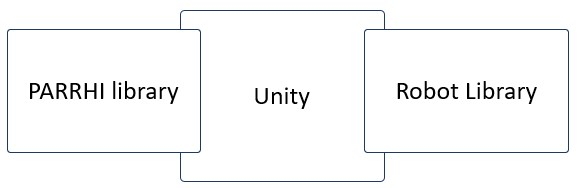
\includegraphics[width=0.5\textwidth]{Figures/Implementation_SystemSetup.jpg}
	\caption{PARRHI implementation setup}
	\label{Fig:Implementation}
\end{figure}


%4.2) PARRHI Library
\section{PARRHI Library}
%- Build up, workflow, interesting things
The PARRHI system was programmed in Microsoft's .NET framework version 4.6.1~\cite{NETFramework} using $C\#$ \cite{CSharp}. Besides being my personal preference, this decision was made because the Unity game engine is used with the language $C\#$. The PARRHI library itself is a \textit{Class Library} project~\cite{ClassLibrary} and has three main tasks.

\begin{enumerate}
	\item Import the Parametrised Program and perform some operations on it. The Parametrised Program is a XML~\cite{xmlW3C} based document. After importing, it is validated using an XSD~\cite{xsdW3C} document. Finally the PARRHI library has to extract useable $C\#$ objects from the deserialized XML document and setup references to resolve parameters.
	\item The Real World Model and the logic behind it is a subcomponent of this library. In my specific case, this means, that the PARRHI library contains the Robot's forward kinematics model and the required information to convert the HoloLens' internal coordinates, into the robot's coordinate system.
	\item The Core Routine is located in the PARRHI library, meaning, that on every iteration the PARRHI system calls into the PARRHI library to perform its task.
\end{enumerate}

Importing and validating the XML document is very easy, since the used .NET framework natively supports that. The implementation of the PARRHI Core Routine is also quite straight forward, which is why I will not talk about it too much. More interesting is the Robot's forwards kinematics, which will be presented now.

\subsection{CR-i7A Forward Kinematics}
In robotics, a robot can be described in two different spaces. On one hand there is the joint space, meaning that all vectors and matrices depend on the joint positions, velocities or accelerations. Since the robot has six joints, the joint space is six dimensional. In the joint space the position vector is often represented as $ \vec{q} $.

On the other hand there is the task-space. In this space, all vectors and matrices depend on the Cartesian position and orientation (and their first two derivations) $ \vec{x}, \dot{\vec{x}}, \ddot{\vec{x}} $ of the robot's TCP. If the joint space is six dimensional, then generally speaking (ignoring cases like singularities) the task space is also six dimensional and represented as follows, with $x,y,z$ being the 3D coordinates, and $\alpha, \beta, \gamma $ being the orientation of the tip.
\[ \vec{q} = \begin{pmatrix} q_1 \\ q_2 \\ q_3 \\ q_4 \\ q_5 \\ q_6 \end{pmatrix}, \vec{x} = \begin{pmatrix} x \\ y \\ z \\ \alpha \\ \beta \\ \gamma \\ \end{pmatrix} with~~\vec{x},\vec{q} \in \mathbb{R}^6  \]

The forward kinematics now describes the process of transitioning form $ \vec{q} $ to $ \vec{x} $. This is done as follows: $ \vec{x} = f(\vec{q})~with~f: \mathbb{R}^6 \rightarrow \mathbb{R}^6$. Where the mapping $f$ depends on the robot's specific configuration and geometric properties. For reference, if $f$ is a mapping from $\mathbb{R}^6 \rightarrow \mathbb{R}^6$ then $f^{-1}$ (if it exists!) with $ \vec{q} = f^{-1}(\vec{x})$ is called inverse kinematics. 

To calculate $f$, I first defined local Cartesian coordinate systems after each joint. In fig.~\ref{Fig:ForwardKinematics} the green axes represent the robot, the black vector packs of three represent the coordinate systems $\phi_i = (x_i, y_i, z_i)$ and $\vec{l}_i$ represent the axes defined in the coordinate system $\phi_i$. In the following paragraph, the notation of  $\vec{l}_{a,b}$ will be used to name the $a^{th}$ vector called $\vec{l}$ expressed in the coordinate system $b$.

\begin{figure}[!h]
	\begin{minipage}{0.45\textwidth}
		\centering
		
\tdplotsetmaincoords{60}{120} 
\begin{tikzpicture}  [scale=0.08, tdplot_main_coords, axis/.style={->, black, thin}, 
vector/.style={-stealth,green,very thick}, 
robot/.style={green, very thick},
vector guide/.style={dashed,gray,thin}]

\usetikzlibrary{calc}

%standard tikz coordinate definition using x, y, z coords
\coordinate (O) at (0,0,0);

%tikz-3dplot coordinate definition using x, y, z coords


\pgfmathsetmacro{\axSize}{100}
\pgfmathsetmacro{\saxSize}{10}
\pgfmathsetmacro{\jointRadius}{30}

%Robot Points in cm (mm too large dimensions for library)
\coordinate (P0) at (0,0,0);
\coordinate (P1) at (5,0,33);
\coordinate (P2) at (5, 0, 77);
\coordinate (P25) at (10, 0, 100.5);
\coordinate (P3) at (15, 0, 100.5);
\coordinate (P4) at (47, 0, 100.5);
\coordinate (P5) at (55, 0, 100.5);
\coordinate (P6) at (63, 0, 100.5);


%draw coordinate system axes
%\draw[axis] (0,0,0) -- (\axSize,0,0) node[anchor=north east]{$x$};
%\draw[axis] (0,0,0) -- (0,\axSize,0) node[anchor=north west]{$y$};
%\draw[axis] (0,0,0) -- (0,0,\axSize) node[anchor=south]{$z$};


\draw[axis] (P0) -- (\saxSize,0,0) node[anchor=north east]{$x_0$};
\draw[axis] (P0) -- (0,\saxSize,0) node[anchor=north west]{$y_0$};
\draw[axis] (P0) -- (0,0,\saxSize) node[anchor=west]{$z_0$};

\draw[axis] (P1) -- ($ (P1) + (\saxSize,0,0)$) node[anchor=north east]{$x_1$};
\draw[axis] (P1) -- ($ (P1) + (0,\saxSize,0)$) node[anchor=north west]{$y_1$};
\draw[axis] (P1) -- ($ (P1) + (0,0,\saxSize)$) node[anchor=west]{$z_1$};

\draw[axis] (P2) -- ($ (P2) + (\saxSize,0,0)$) node[anchor=north east]{$x_2$};
\draw[axis] (P2) -- ($ (P2) + (0,\saxSize,0)$) node[anchor=north]{$y_2$};
\draw[axis] (P2) -- ($ (P2) + (0,0,\saxSize)$) node[anchor=south]{$z_2$};

\draw[axis] (P3) -- ($ (P3) + (\saxSize,0,0)$) node[anchor=south east]{$x_3$};
\draw[axis] (P3) -- ($ (P3) + (0,\saxSize,0)$) node[anchor=north west]{$y_3$};
\draw[axis] (P3) -- ($ (P3) + (0,0,\saxSize)$) node[anchor=south]{$z_3$};

\draw[axis] (P4) -- ($ (P4) + (\saxSize,0,0)$) node[anchor=south east]{$x_4$};
\draw[axis] (P4) -- ($ (P4) + (0,\saxSize,0)$) node[anchor=south west]{$y_4$};
\draw[axis] (P4) -- ($ (P4) + (0,0,\saxSize)$) node[anchor=south]{$z_4$};

\draw[axis] (P5) -- ($ (P5) + (\saxSize,0,0)$) node[anchor=north east]{$x_5$};
\draw[axis] (P5) -- ($ (P5) + (0,\saxSize,0)$) node[anchor=north east]{$y_5$};
\draw[axis] (P5) -- ($ (P5) + (0,0,\saxSize)$) node[anchor=south]{$z_5$};

%draw the robot's joints and axes
\draw[robot] (P0) -- (P1); \fill[fill=gray] (P0) circle (\jointRadius pt);
\draw[robot] (P1) -- (P2); \fill[fill=gray] (P1) circle (\jointRadius pt);
\draw[robot] (P2) -- (P25); \fill[fill=gray] (P2) circle (\jointRadius pt);
\draw[robot] (P25) -- (P3); 
\draw[robot] (P3) -- (P4); \fill[fill=gray] (P3) circle (\jointRadius pt);
\draw[robot] (P4) -- (P5); \fill[fill=gray] (P4) circle (\jointRadius pt);
\draw[robot] (P5) -- (P6); \fill[fill=gray] (P5) circle (\jointRadius pt);

%draw the 
\node[tdplot_main_coords,anchor=east] at ($(P0) + (10,0,15)$){$\vec{l_0}$};
\node[tdplot_main_coords,anchor=east] at ($(P1) + (5,0,20)$){$\vec{l_1}$};
\node[tdplot_main_coords,anchor=east] at ($(P2) + (-12,0,00)$){$\vec{l_2}$};
\node[tdplot_main_coords,anchor=east] at ($(P3) + (10,0,10)$){$\vec{l_3}$};
\node[tdplot_main_coords,anchor=south east] at ($(P4) + (-1,1,0)$){$\vec{l_4}$};
\node[tdplot_main_coords,anchor=north] at ($(P5) + (0,0,0)$){$\vec{l_5}$};




\end{tikzpicture}
		\caption{Robot forward kinematics\\coordinate systems}
		\label{Fig:ForwardKinematics}
	\end{minipage}\hfill
	\begin{minipage}{0.45\textwidth}
		The matrix ($\phi_{n+1}$) allows the conversion from vectors expressed in the coordinate system $n + 1$ to the expression in system $n$, with $\vec{l}_{n+1,n} = \phi_{n+1}(q_{n+1}) * \vec{l}_{n+1,n+1}$. After transforming the vector $\vec{l}_{n+1}$ one can add the vector $\vec{l}_{n,n}$ because they are both defined in the same coordinate system. Meaning, that the position of the tip of the vector $\vec{l}_{n+1}$ relative to the origin of the coordinate system $n$ is, $\vec{x}_{n+1,n} = \phi_{n+1}(q_{n+1}) * \vec{l}_{n+1,n+1} + \vec{l}_{n,n} $.\\
		Repeating this process from $n = 5$ to $n = 0$, results in the robot's TCP position relative to the coordinate system $\vec{O}$, which is what we wanted. One has to remember, that only the matrices $\phi_{i}$ are variables, since they depend on $q_i$. The vectors $\vec{l}_i$ are constants. This means, that for each iteration one only has to calculate all matrices $\phi_i$ and can then calculate the positions $(x_i, y_i, z_i)$ of each coordinate system relative to the base system $\vec{O}$.
	\end{minipage}
\end{figure}

\FloatBarrier

Since the $C\#$ implementation of this algorithm is only about 20 lines of code (excluding the definitions of the matrices $\phi_i$ and the vectors $\vec{l}_i$), takes only about 4ns to run, and the end results are all joint positions in Cartesian coordinates relative to a base system, I am quite happy with the outcome. If one wanted to add multiple robots into this framework, it could be done quite easily by adding one additional world-coordinate system, where all robot base systems are embedded into.
	
Adjusting this model to other types of robots would be easy. If the adjusted joints are all 1 DOF and rotational, then only the rotation matrix $\phi_i$ has to be adjusted, and $\vec{l}_i$ still stays constant. If one included translational, linear joints, the vector $\vec{l}_i$ would depend on some variable, but the mathematical process would stay the same.

Implementation wise one interesting fact is, that Unity (the game engine which hosts the PARRHI library) uses a left-hand coordinate system, whereas my robot forward kinematics was done in a right handed system since that is how I learned it the past few years. This means, that the last step in the forward kinematics is, to transform all produced vectors into Unity's coordinate system, which is rather easy. I only needed to swap the $z$ and $y$ coordinates of each joint position.

For further reading into this topic see~\cite{murray2017mathematical}.
	
%4.3) Unity structure
\section{Unity}
%- What is unity?
Unity is the host of the PARRHI and Robot libraries. Originally, Unity itself is a game engine that helps developers to develop, publish, maintain and market their games~\cite{Unity}. Within recent years the company behind Unity, called Unity Technologies, made efforts to become a de facto standard for AR and VR development. Although there are other engines that have similar capabilities, I chose Unity, since I already had two years of experience while working at the chair of Automation and Information Systems at TUM, and because it is scripted in $C\#$. 

There are a lot of third party products for Unity that help the developer with image tracking and general AR interaction. The next paragraphs explain what libraries, and tools where used to handle hand gesture recognition and image tracking.

%4.3.1) General Setup
%\subsection{General Unity Setup}
%- How is library implemented


%4.3.2) Image Tracking
\subsection{Image Tracking}
%- Vuforia Engine
For Image Tacking I used the Vuforia Engine~\cite{Vuforia}. This engine had a rather simple setup in Unity and worked relatively seamlessly in Unity. Compared to other engines and libraries the Vuforia Engine first of all worked, had a good documentation and a user friendly configuration. An important aspect is, that for non-commercial use it is free of charge. 

The PARRHI implementation makes use of two image markers. One of them is attached directly at the robot's base and is of course used to synchronise the Real World with the majority of the AR World. Since the centre of origin of the robot was not at its base, but about 30 cm above the first joint, there is a small translation between the image markers position and the AR World's coordinate system. The second image marker is used to display the User's UI. The User is given a small sheet of paper with the said image on it, and the PARRHI system projects the User's tasks, some configuration and debug options onto it.


%4.3.3) ARToolkit%
\subsection{AR-Toolkit}
%- AR Toolkit explanation and usage
Interacting with Augmented Reality objects is an essential part of AR environments. Fortunately, Microsoft's open sourced Mixed Reality Toolkit~\cite{MicrosoftMRToolkit} makes this an easy task. The library directly integrates into the Unity environment and allows easy hand gesture recognition (pinching) for clicking and pointing at objects in the augmented space. Since both the HoloLens and the Mixed Reality Toolkit are developed by Microsoft, the library utilises all features and allows for an easy integration.


%4.4) Robot Protocol
\section{Robot Library}\label{Section:RobotLibrary}
%- Strucutre, languages, problems, solutions
Next to the PARRHI library and Unity, the Robot library is the big third component in the PARRHI implementation. The following chapter will explain how we accessed the controller's data, transferred the data to the HoloLens and generally communicated with the robot. The whole Robot library was built together with Florian Leitner, who is currently writing his bachelor's thesis about a virtual programming environment of industrial robots at the same chair as I am. Since his thesis is being written at this very moment, I cannot reference to any source of his.

The Robot Library is responsible for the communication between any system that is capable of executing .NET framework applications, and the robot's controller R-30iB~(see section~\ref{Section:PARRHIHardware}). It is important to know, that Fanuc's controllers are not easily controllable by non-Fanuc components. Our goal was, to wirelessly control the robot from external devices that run .NET framework applications. Since there where no "plug and play" solutions available, we came up with the system, that will be explained in the rest of this chapter. As it has been done in the concept chapter, I will first shortly explain each component before elaborating on the information flow between them. Finally, I will give some details about the implemented, custom protocol we use. Fig.~\ref{Fig:RobotArchitecture} depicts how the system is actually setup.

\begin{figure}
	\centering
	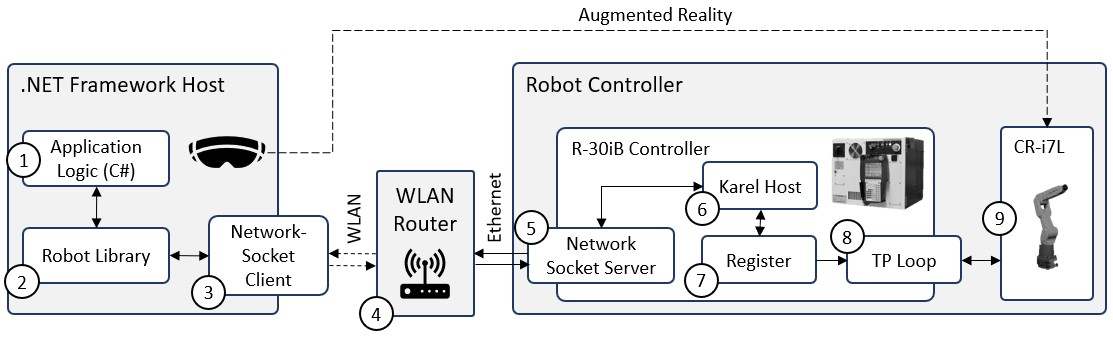
\includegraphics[width=1\textwidth]{Figures/RobotArchitecture.jpg}
	\caption{Robot library setup}
	\label{Fig:RobotArchitecture}
\end{figure}

\begin{enumerate}
	\item Application Logic: This is any application that wants to communicate with the robot. In my case the PARRHI system.
	\item Robot Library: A custom library written in $C\#$ that offers some wrappers around our custom protocol, which simply is a syntax we defined to transfer commands and data over the Network Socket, that follows certain rules, so that both the KAREL Host and the $C\#$ Library can parse them for the important information.
	\item Network Socket Client: Standard Network Socket, where the PARRHI library represents the client.
	\item WLAN Router: Standard WLan Router, which is connected to the controller via a CAT cable.
	\item Network Socket Server: Standard Network Socket, where the Controller represents the server.
	\item KAREL Host: A programm written in KAREL~\cite{FanucKarel} that receives commands from the network socket, parses them according to the defined protocol and returns the requested data or executes the requested commands.
	\item Register: A storage that is used to command the Teach Pendant (TP) Loop, which also has access to this storage location. Some registers are used to set different modes like coordinate systems, absolute versus relative and so on, and six registers are used to transfer vectors, that the TP program should process according to the set mode.
	\item TP Loop: A program written in TP that scans the Register (7) each cycle, and controls the robot accordingly.
\end{enumerate}

Since researching the difference between KAREL and TP programmes on the internet is rather hard, because one simply does not find a lot of information about it, I would like to summarise our current knowledge about that. KAREL is a programming language, that is similar to Fortran. It was developed by Fanuc itself, and is used internally for alot of components in the controller. Nowadays, KAREL is most often used for managing tasks like communication, synchronisation, data handling and so on. Teach pendant programmes on the other hand, are specialised on actually commanding the robot's movement and behaviour. TP supports numerous methods to control a robot, that the KAREL language simply does not offer. This is why, we chose to split up the controller-side software in these two programming components.

Now the information flow happens as follows: First, the Application (1), which wants to send a command to the robot has to call into the Robot Library (2). Besides managing the Network Socket Connection (3), this library offers about 10 commands to the Application. A command could be the wish to fetch the robot's joint position, or to move the robot into a certain position. The Robot Library (2) then sends the command to the Network Socket (3), which is connected to the controllers server-endpoint. It is important, that the communication between the HoloLens (or a Laptop for instance) is wireless in order to stay mobile. The controller is connected to the WLAN Router (4) via a cable using the Ethernet protocol. There, the Network Socket Server (5) receives the command, and passes it on to the KAREL Host (6). 

At this point the command is only a string following a very specific syntax that we defined. The Karel Host (6) then parses the command and acts on its instructions. If the command is a simple "Fetch Command", the Karel Host (6) collects the needed data, constructs the message and sends it back via the network. If the command is targeted at the robot itself, the Karel Host (6) fills the Register (7) with all necessary data that the TP Loop (8) needs to execute the movement command. This data is a six dimensional vector (TCP coordinates in task space) and the mode whether the vector should be interpreted absolute or relatively to the momentary position.

Basically, the presented architecture allows us to execute any pre-defined function in a fraction of a second. The whole process is actually so fast, that the PARRHI system fetches the robot's joint position in each iteration.

To finish this chapter off, I would like to shortly explain what the system is capable of doing. The Robot Library can get the robot's joint angles, TCP position and six dimensional force/torque sensor data. It can command the robot to drive to an absolute or relative task or joint space position and set a speed vector for the TCP. Generally, this system could be extended quite easily.

%4.5) Parametrised Program Validation and Definition
\section{Parametrised Program Implementation and Validation}
%- XML leads to C# classes etc.
One last interesting component in the PARRHI implementation is the Parametrised Program. It was clear quite early on, that the document needs a hierarchical structure and must be validated, since the PARRHI system has some presupposed assumptions about the document.  

XML~\cite{xmlW3C} immediately comes into mind here. XML documents are strictly hierarchically and have the big benefit of being human and machine readable. In PARRHI's case this is exactly what the document in question should be. Written by a human with limited software engineering skills, but interpreted by a machine.


%4.4.1) XML Structure
\subsection{Parametrised Program XML Structure}
%%- Give XML Tags
The content of the Parametrised Program was thoroughly discussed in section~\ref{Section:ParametrisedProgram}. In this section, I would like to present the actual implementation and how a Parametrised Program written in XML would look like.

XML documents must have one root element. In PARRHI's case this is the "<PProgram/>" tag. Similarly to the conceptual train of thought, the actual implementation contains four sub elements.

\begin{lstlisting}
<?xml version="1.0"?>
<PProgram xmlns="PARRHI">
	<Variables>...</Variables>
	<Points>...</Points>
	<Holograms>...</Holograms>
	<Events>
		<Trigger>...</Trigger>
		<Actions>...</Actions>
	</Events>
</PProgram>
\end{lstlisting}

Each child element of PProgram can now take their object definitions directly. Only the "Events" element categorises its content in two sub elements "Triggers" and "Actions". It is important to know, that every object defined in the Parametrised Program has to have a unique name attribute to identify it in other parts of the application. 

The following block of code exemplary defines each object once. Please note, that this program is not written to actually do something meaningful, it only presents all ways to define objects in the Parametrised Program. Of course the Developer could use every object multiple times and also create multiple instances of the same object types, as long as their name is unique.

\begin{lstlisting}
<?xml version="1.0"?>
<PProgram xmlns="PARRHI">
	<Variables>
		<Int name="Variable0">0</Int>
	</Variables>
	<Points>
		<PointCamera name="CamPoint"/>
		<PointFix name="FixPoint0" X="200" Y="-300" Z="300" />
		<PointRobot name="RobotPoint0" J1="1" J2="2" Scale="0.6" />
	</Points>
	<Holograms>
		<Cylinder name="Cyl0" point1="CamPoint" point2="FixPoint0" radius="10" active='false'/>
		<Sphere name="Sphere0" point="RobotPoint0" radius="25" renderMode="transparent" active='true'/>
	</Holograms>
	<Events>
		<Trigger>
			<DistanceTrigger name="DistanceTrigger0" canTrigger='true' point1="CamPoint" point2="RobotPoint0" distance="15.5" action1="HoloStateAction0"/>
			<VarTrigger name="VariableTrigger0" canTrigger='true' varName="Variable0" triggerValue="2" action1="IncrVarAction0"/>
			<TimeTrigger name="TimeTrigger0" canTrigger='true' timeSinceActivation="120" action1="TriggerStateAction0" action2="ChangeUITextAction0"/>
		</Trigger>
		<Actions>
			<IncrementCounterAction name="IncrVarAction0" intVar="Variable0"/>
			<SetHologramStateAction name="HoloStateAction0" state='true' holograms="Zyl1 Sphere1 Sphere2 Zyl2"/>
			<SetTriggerStateAction name="TriggerStateAction0" triggerName="Trigger1" canTrigger='true'/>
			<ChangeUITextAction name="ChangeUITextAction0" text="Tutorial step nr. 4"/>
			<MoveRobotAction name="MoveRobotAction0" pointTCP="FixPoint0" />
			<SetRobotHandStateAction name="SetRobotHandAction0" state="open" />
		</Actions>
	</Events>
</PProgram>
\end{lstlisting}

It does not matter in which sequence all the elements occur. Only the hierarchically structure has to be kept exactly as the example document above. The PARRHI library will at some point deserialise the Parametrised Program using a standard .NET Framework XML library. For this deserialisation a validation should be performed, in order to find flaws beforehand.

%4.4.2) XSD generation and validation#
\subsection{XSD generation and validation}
%- Auto generate xsd and c# classes
The hierarchy of XML documents can be specified very detailed in XML-scheme documents, which are also called XSD files~\cite{xsdW3C}. These documents define which element can or must occur at witch location in the XML document, which attributes these elements can or must have and so on. The XSD file can even specify minimum and maximum values, data types and much more.

Hence, an XSD document is an essential part in the importing / validation process. Since writing these documents can be enormously work intensive, Microsoft has developed ways to generate XML schemes from a set of XML documents. Especially, when the underlying XML document may change repeatedly, it can be very exhausting to update the XSD file every time. For that I wrote a small $C\#$ application, that takes multiple .xml documents as an input, and outputs one XSD document that defines rules, which fit to all input XML files. 

Another application developed by Microsoft called "xsd.exe"~\cite{xsdExe} allows to convert XSD documents into $C\#$ class definitions. During the development of this bachelor's thesis, I automated the process of generating the XSD file and from that the $C\#$ class definition, using the programming language Perl~\cite{perl}.

This means, that whenever I wanted to add an attribute to some xml element in the Parametrised Program, I only had to add these attributes in one of my example input xml documents and execute the Perl script, which would then output new XSD documents and a $C\#$ class to deserialise the Parametrised Program. 

One huge advantage of XSD documents and their validator is, that the latter can output exact error messages with what went wrong in the input xml document. This includes the type of error, line and column numbers, and (depending on the error type) suggests how to fix it. For the PARRHI system this means, that very exact feedback can be printed to the user if any errors occur. This makes it easier for non software engineers to accomplish their task.




















